% This file was created by tikzplotlib v0.9.8.
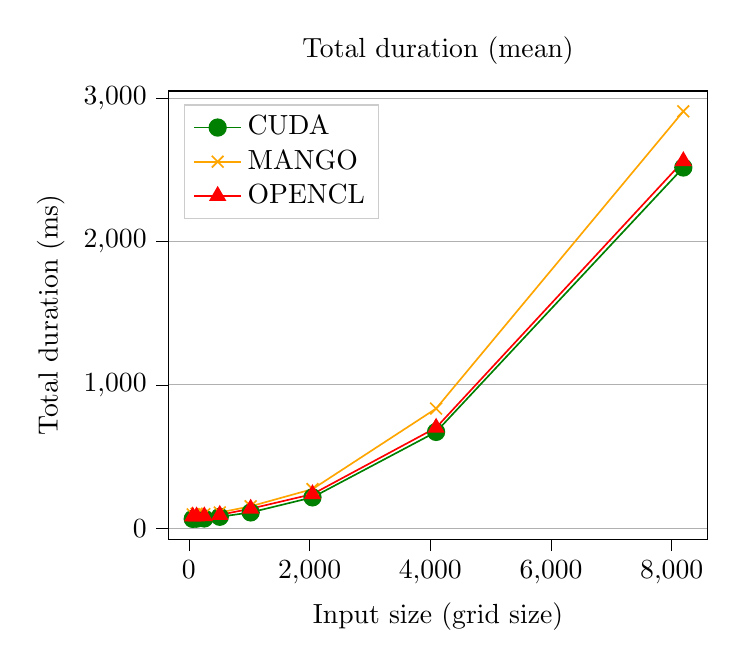
\begin{tikzpicture}

\definecolor{color0}{rgb}{1,0.647058823529412,0}

\begin{axis}[
legend cell align={left},
legend style={
  fill opacity=1,
  draw opacity=1,
  text opacity=1,
  at={(0.03,0.97)},
  anchor=north west,
  draw=white!80!black
},
tick align=outside,
tick pos=left,
title={Total duration (mean)},
x grid style={white!69.0196078431373!black},
xlabel={Input size (grid size)},
xmin=-342.4, xmax=8598.4,
xtick style={color=black},
y grid style={white!69.0196078431373!black},
ylabel={Total duration (ms)},
ymajorgrids,
ymin=-76.746247884394, ymax=3050.06359712783,
ytick style={color=black},
scaled x ticks = false,
xtick={0, 2000, 4000, 6000, 8000},
]
\addplot [semithick, green!50.1960784313725!black, mark=*, mark size=3, mark options={solid}]
table {%
64 65.3814723434343
128 67.1212662244898
256 68.3322663666667
512 80.0275030333333
1024 110.4768081
2048 215.540796947368
4096 671.9512696
8192 2516.1915956
};
\addlegendentry{CUDA}
\addplot [semithick, color0, mark=x, mark size=3, mark options={solid}]
table {%
64 96.4079058736842
128 101.54462224
256 98.3502921071428
512 109.975305
1024 153.2529195
2048 272.943125684211
4096 834.9055927
8192 2907.9358769
};
\addlegendentry{MANGO}
\addplot [semithick, red, mark=triangle*, mark size=3, mark options={solid}]
table {%
64 82.7704575208333
128 82.79732128
256 83.8056829333333
512 93.437536862069
1024 136.60162595
2048 237.940542842105
4096 701.5180952
8192 2561.3243602
};
\addlegendentry{OPENCL}
\end{axis}

\end{tikzpicture}
